\chapter{Modello teorico di Controllo}\label{cap:controlModel}

\begin{minipage}{12cm}\textit{In questo capitolo viene affrontato il problema della creazione di un controllo lineare per l'impianto, che permetta di raggiungere un inseguimento a errore nullo per l'uscita.}
\end{minipage}

\vspace*{1cm}

\section{Obiettivo di controllo}
Come accennato nella sezione "\nameref{sub:parametriMisurati}", attraverso il controllo e attuazione della corrente del Trasformatore, si punta controllare la corrente di Plasma, qui rappresentata caso dalla corrente sul Secondario del trasformatore, e come si è già fatto osservare nella medesima sezione, non essendo possibile misurare nella realtà la corrente di Plasma con metodi diretti, si usa come misura indiretta la $ V_{loop} $ ($ F_{em} $ nel nostro esperimento).\\
In questa tesi l'obiettivo di controllo è l'inseguimento a errore nullo del riferimento costante per la corrente di Plasma.\vspace{-4mm}
\begin{figure}[H]
	\centering
	\caption[Sistema da controllare a blocchi con $ P(s) $]{Sistema da controllare a blocchi con $ P(s) $}
	\vspace{1mm}
	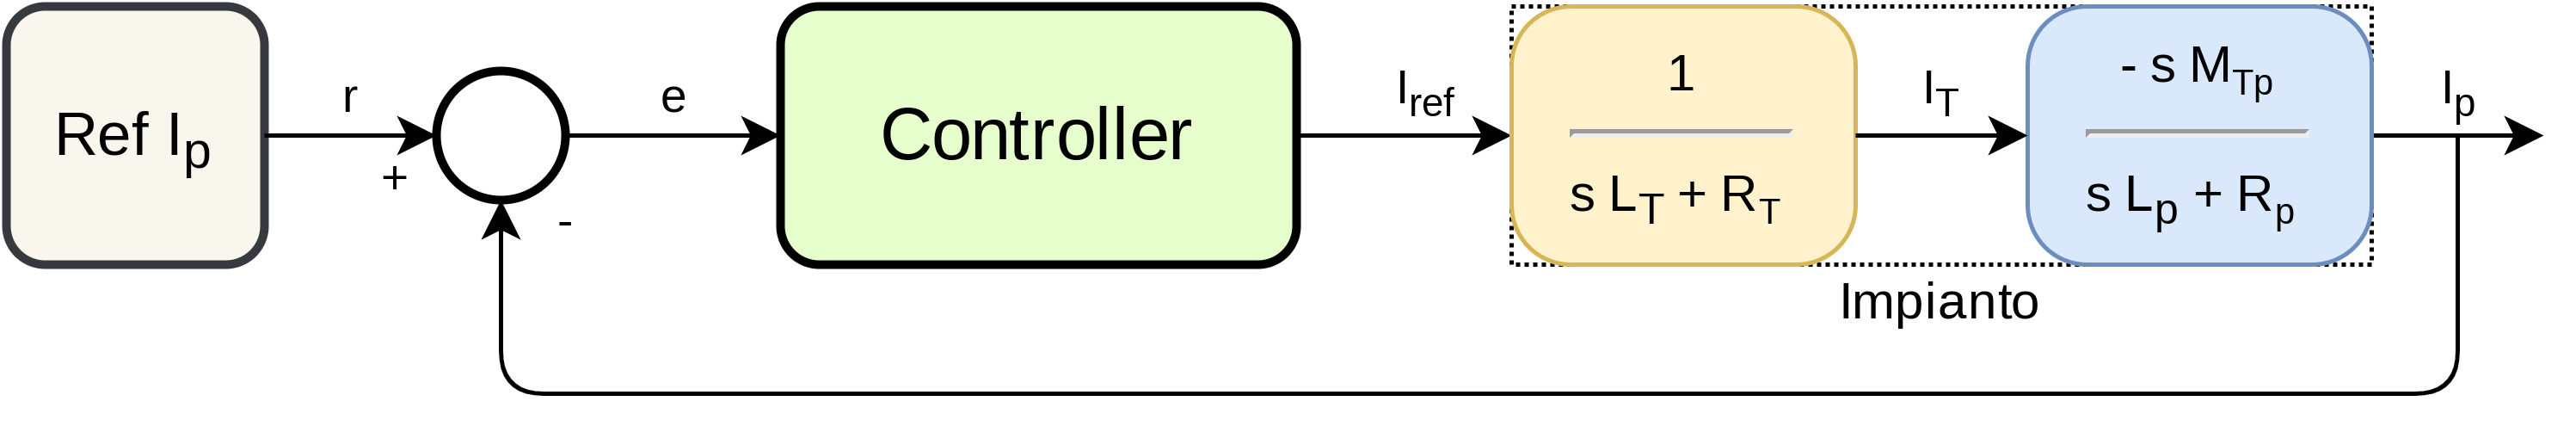
\includegraphics[width=1\textwidth]{ModelloMatematico/SchemiBlocchi.png}
\end{figure}\vspace{-4mm}

\noindent
La misura a nostra disposizione è però la tensione letta dal voltmetro $V_2$ ($ \Rightarrow F_{em}$ nel nostro caso, $V_{loop} $ in un impianto reale).\\
Dall'equazione della dinamica del plasma \ref{eq:correntePlasmaDinamica} siamo in grado di ricavare che:
\begin{empheq}[box=\mathStep]{equation*}
	V_2 = I_p \cdot R_p = F_{em} - L_p \cdot \dot{I_p}
\end{empheq}

\noindent
Dalla quale, trascurando la dinamica del filtro RC di misura (che comunque è $ \ge$ della frequenza di campionamento $ f_{tic} (2Khz) $ e di conseguenza ha una dinamica estremamente più rapida del segnale da misurare, quindi trascurabile),  permette di ricavare, la funzione di trasferimento che lega l'ingresso $ I_{ref} $ all'uscita $ V_2 $ \footnote{Nota bene, la $ V_2 $ è misurata in realtà invertendo i poli del trasformatore, e quindi il segno di uscita, mettendoci di conseguenza nella situazione di avere $ P_{pos} $ come funzione di trasferimento} ,ed essa risulta essere:
\begin{empheq}[box=\mathCalc]{equation}
	V_2(s) = I_p(s) \cdot- R_p \Rightarrow V_2(s) = P_{pos}(s) \cdot I_{ref}(s) \cdot R_p
\end{empheq}
Da cui la funzione di trasferimento complessiva diventa:
\begin{empheq}[box=\mathCalc]{equation}\label{eq:FunxTrasImpiantoIrefV2}
	\frac{V_2(s)}{I_{ref}(s)} = P_{pos}(s) \cdot R_p
\end{empheq}
E il riferimento di corrente di plasma, diventa un riferimento di tensione secondo l'equazione di conversione:
\begin{empheq}[box=\mathCalc]{equation}\label{eq:V2RefEquivalent}
	V_{2_{ref}} = I_{p_{ref}} \cdot R_p
\end{empheq}

\begin{figure}[H]
	\centering
	\caption[Sistema da controllare ingresso-uscita reale]{Sistema da controllare ingresso-uscita reale}
	\vspace{1mm}
	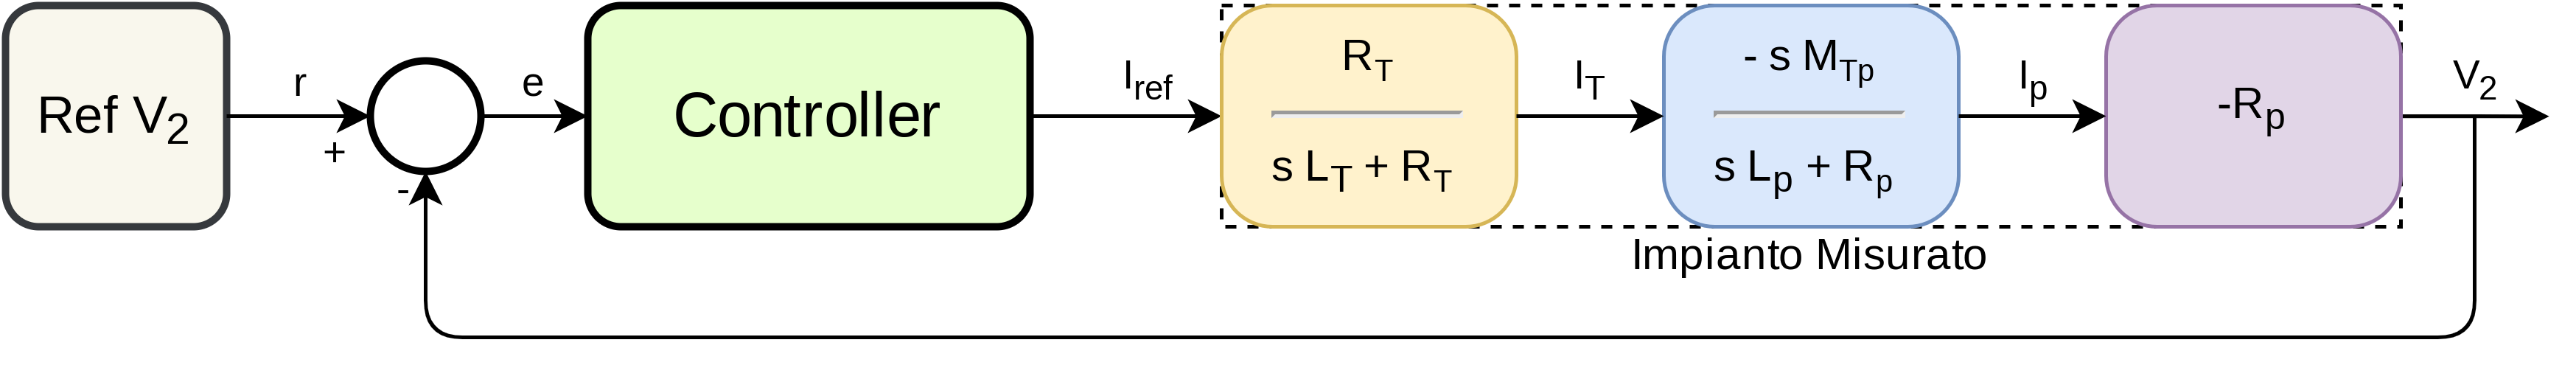
\includegraphics[width=1\textwidth]{ModelloMatematico/SchemiBlocchi-SchemaBlocchiV2Out.png}
\end{figure}

\newpage
\section{Teorema del valore iniziale e del valore finale}
Prima di procedere con il calcolo del controllore per i nostri scopi, è bene ricordare il \nameref{th:valIniziale} e il \nameref{th:valFinale} della Trasformata di Laplace (\cite*{Laplace}):

\begin{teorema}[Teorema del valore iniziale \label{th:valIniziale}]
	Se una funzione reale $ f  $ ha trasformata razionale $ F(s) $ con grado del denominatore maggiore del grado del numeratore (vale comunque sotto ipotesi ancora più larghe , purché $ F $ sia non razionale e $ f(0^+) $ esista) allora:
	\begin{empheq}[box=\mathResult]{equation} \label{eq:valIniziale}
		f(0^+) = \lim\limits_{s \rightarrowtail \infty} s \cdot F(s)
	\end{empheq}
\end{teorema}

\begin{teorema}[Teorema del valore finale \label{th:valFinale}]
	Se una funzione reale $ f  $ ha trasformata razionale $ F(s) $ con grado del denominatore maggiore del grado del numeratore e \underline{radici del denominatore (\textbf{poli}) nell’origine e o a parte reale negativa},\\
	allora:
	\begin{empheq}[box=\mathResult]{equation} \label{eq:valFinale}
		\lim\limits_{t \rightarrowtail \infty} f(t) = \lim\limits_{s \rightarrowtail 0} s \cdot F(s)
	\end{empheq}
\end{teorema}

Questi 2 Teoremi chiave, permettono di risolvere comodamente le equazioni differenziali, e quindi calcolare in maniera semplice il controllore che permette di ottenere gli obiettivi di controllo che ci si è prefissati di ottenere.

\newpage

\section{Controllo a errore nullo} \label{sec:inseguitoreErroreNullo}
\vspace{-5mm}
Definiamo ora $ P_m(s) $ come l'impianto Reale misurato tra la corrente di riferimento $ I_{ref} $ del primario, e la tensione del campo elettrico $ V_2 $ sul secondario.
\begin{empheq}[box=\mathCalc]{equation}\label{eq:impiantoMisurato}
	P_m(s)= \frac{V_2(s)}{I_{ref}(s)} = \frac{s M_{Tp} \cdot R_p}{( s L_p + R_p)(s L_T + R_T)} = \frac{s M_{Tp} \cdot R_p}{s^ 2L_p L_T + s(L_p R_T + L_T R_p) + R_p R_T}
\end{empheq}
Essendo il nostro obiettivo quello di portare $ e \rightarrowtail 0$ per $ t\rightarrowtail \infty $ con riferimenti $ r = K_r \in \mathbb{R} $, usando la funzione sensitività $ W_{er}(s) $ e  il \nameref{th:valFinale} per inferire sull'evoluzione della dinamica di errore a \textit{steady state} , progetteremo il controllore $ C(s) $ che permetta di realizza l'obiettivo $ e \rightarrowtail 0$:\\
\begin{vwcol}[widths={0.5,0.5}, sep=8mm, rule=0px]
	\vspace{-12mm}
	\begin{empheq}[box=\mathStep]{equation*}
		W_{er}(s) = \frac{e(s)}{r(s)} = \frac{1}{1 + P_m(s)C(s)}
	\end{empheq}
	\newpage
	{\color{red} Sensitivity transfer function}\\[-6mm]
	{\footnotesize (\cite{PerfAndRobust})}
\end{vwcol}
\vspace{5mm}
\begin{vwcol}[widths={0.5,0.5}, sep=8mm, rule=0px]
	\vspace{-8mm}
	\begin{empheq}[box=\mathStep]{equation*}
		r(t) = K_r \in \mathbb{R} \rightarrow r(s)= \frac{K_r}{s}
	\end{empheq}
	\newpage
	Trasformata di Laplace del riferimento
\end{vwcol}\vspace{-3mm}
\noindent
Da cui, applicando il \nameref{th:valFinale} otteniamo:
\begin{empheq}[box=\mathCalc]{equation} \label{eq:dinamicaErroreRifCostFunxTrasf}
	\lim\limits_{t \rightarrowtail \infty} e(t) = \lim\limits_{s \rightarrowtail 0} s \cdot W_{er}(s) \cdot r(s) = s \cdot \frac{K_r / s}{1 + P_m(s)C(s)}
\end{empheq}

\begin{oss} \label{oss:Fattorizzazione}
	Al fine di semplificare i calcoli per la realizzazione del design del controllore, fattorizziamo ora $ P_m(s) $ e $ C(s) $ nella seguente forma polinomiale frazionaria, tralasciando così i dettagli dei termini non utili ai fini del design del controllore.\\[0mm]
	\begin{vwcol}[widths={9cm,4cm}, sep=0mm, rule=0px]
		\vspace{-8mm}
		\begin{empheq}[box=\mathStep]{equation*}
			C(s) = K_c \cdot \frac{s^{\rho_{c_n}} \cdot \prod_{i=1}^{\#Zeri\neq0} \left ( \frac{s}{z_i} + 1 \right )}{s^{\rho_{c_d}} \cdot \prod_{i=1}^{\#Zeri\neq0} \left ( \frac{s}{p_i} + 1 \right )} =
			\frac{K_c}{s^{\rho_{c}}} \cdot \frac{C_n(s)}{C_d(s)}
		\end{empheq}
		\newpage
		\begin{spacing}{1.25}
			{\scriptsize
				\begin{itemize}[itemsep=-1mm,leftmargin=6mm]
					\item $ K_c $ Guadagno statico Controllore.
					\item $ C_n $ Polinomio numeratore \underline{senza Zeri in 0}.
					\item $ C_d $ Polinomio denominatore \underline{senza Poli 0}.
					\item $ \rho_c $ è il grado del polo in 0 ($ \rho_{c_d} - \rho_{c_n} $).
				\end{itemize}
			}
		\end{spacing}
	\end{vwcol}

	\noindent\rule[0.5ex]{\linewidth}{0.5pt}\\[0mm]

	\begin{vwcol}[widths={9cm,4cm}, sep=0mm, rule=0px]
		\vspace{-10mm}
		\begin{empheq}[box=\mathStep]{equation*}
			P(s) = K_p \cdot \frac{s^{\rho_{p_n}} \cdot \prod_{i=1}^{\#Zeri\neq0} \left ( \frac{s}{z_i} + 1 \right )}{s^{\rho_{p_d}} \cdot \prod_{i=1}^{\#Zeri\neq0} \left ( \frac{s}{p_i} + 1 \right )} =
			\frac{K_p}{s^{\rho_{p}}} \cdot \frac{P_n(s)}{P_d(s)}
		\end{empheq}
		\newpage
		\begin{spacing}{1.25}
			{\scriptsize
				\begin{itemize}[itemsep=-1mm,leftmargin=6mm]
					\item $ K_p $ Guadagno statico Impianto.
					\item $ P_n $ Polinomio numeratore \underline{senza Zeri in 0}.
					\item $ P_d $ Polinomio denominatore \underline{senza Poli 0}.
					\item $ \rho_p $ è il grado del polo in 0 ($ \rho_{p_d} - \rho_{p_n} $).
				\end{itemize}
			}
		\end{spacing}
	\end{vwcol}
\end{oss}
\newpage
Usando la forma nell'osservazione \ref{oss:Fattorizzazione}da questa forma, svolgiamo i calcoli dell'equazione  \ref{eq:dinamicaErroreRifCostFunxTrasf}:
\begin{empheq}[box=\mathCalc]{equation} \label{eq:guadagnoAnelloPlusOne}
	1 + P_m(s)C(s) =  1 + \frac{K_c}{s^{\rho_{c}}} \frac{C_n}{C_d}\cdot \frac{K_p}{s^{\rho_{p}}}  \frac{P_n}{P_d}=
	\frac{s^{\rho_{c} + \rho_{p}} C_d P_d + K_c K_p C_n P_n}{s^{\rho_{c} + \rho_{p}} C_d P_d}
\end{empheq}

Da cui otteniamo che:
\begin{center}
	{\large
		$ s \cdot W_{er}(s) \cdot r(s) =
			\cancel{s} \cdot \frac{K_r/\cancel{s}}{1 + P_m(s)C(s)} =
			K_r \cdot \left(\frac{s^{\rho_{c} + \rho_{p}} C_d P_d + K_c K_p C_n P_n}{s^{\rho_{c} + \rho_{p}} C_d P_d}\right)^{-1} \Rightarrow$
	}
\end{center}

\begin{empheq}[box=\mathStep]{equation*}
	\lim\limits_{t \rightarrowtail \infty} e(t) = \lim\limits_{s \rightarrowtail 0} s \cdot W_{er}(s) \cdot r(s) = \lim\limits_{s \rightarrowtail 0}
	K_r \cdot \frac{{\color{fireenginered}s^{\rho_{c} + \rho_{p}}} \cdot C_d P_d}{{\color{fireenginered}s^{\rho_{c} + \rho_{p}}} \cdot C_d P_d + K_c K_p C_n P_n}
\end{empheq}
Tenendo presente che $ C_d,P_d,C_n,P_n \rightarrowtail 1 $ per $ s \rightarrowtail 0 $, poiché gli Zeri sono stati fattorizzati fuori assieme al guadagno Statico (vedi osservazione \ref{oss:Fattorizzazione}), abbiamo che gli esiti per l'errore a \textit{Steady state} (Stato Stazionario) dipendono solo dal grado di $ s^\rho $ con  {\color{fireenginered}$ \rho = \rho_{c} + \rho_{p} $} e {\color{fireenginered}$\rho \in \mathbb{Z} $}:

\begin{center}	\label{eq:esitiErrore}
	$ e_\infty = \lim\limits_{t \rightarrowtail \infty} e(t) =
		\left \{ \begin{array}{l c c}
			0                   & se & \rho \geq 1 \\
			\frac{K_r}{K_c K_p} & se & \rho = 0    \\
			\infty              & se & \rho \leq 0
		\end{array}
		\right.
	$
\end{center}
Essendo {\color{fireenginered}$ \rho_{p} = -1 $} a causa dello Zero nell'origine dovuto al Trasformatore, segue che il controllore dovrà necessariamente avere 2 poli nell'origine ($ \rho_{c} = 2 $) per ottenere {\color{fireenginered}$ \rho = 1 $}.\\
Da cui, il design base del controllore è: \vspace{-4mm}
\begin{empheq}[box=\mathStep]{equation}	\label{eq:contollerDesignBase}
	C(s) = \frac{1}{s^2}
\end{empheq}\vspace{-2mm}
Questo controllore base è complicabile a piacere aggiungendo altri Poli e Zeri stabili, con l'obiettivo di migliorarne le performance della risposta del sistema.
\begin{oss}
	Il controllore descritto in \ref{eq:contollerDesignBase}, anche se stabilizza il sistema e lo rende un \underline{inseguitore ad errore nullo}, \textbf{non è stabile}! Esso infatti ha 2 poli in 0, rendendolo un polo \textit{non semplice} e quindi causa di instabilità polinomiale.\\
	L'uso di un simile controllore, anche se stabilizza l'uscita del sistema a ciclo chiuso, lo rende al contempo \textbf{Input-to-state \underline{un}stability}.\\
	Questa conseguenza è inevitabile ma bene accetta poiché permette di inseguire con errore nullo, per la durata dell'esperimento, il riferimento, e la presenza di saturazione nell'attuazione evita il problema.\\
	Bisognerà ovviamente tenerne conto in fase di realizzazione poiché con il procedere del tempo dell'esperimento, i numeri dello stato diventeranno sempre maggiori, e ciò potrà portare a problemi di overflow numerici che devono essere gestiti in fase di progettazione del codice.
\end{oss}

\newpage
\noindent
La dinamica $ e_\infty $ riportata (\ref{eq:esitiErrore}) è valida $\leftrightarrow$ il sistema a ciclo chiuso $ W_{V_2 r}(s) $ risulta A.S.\footnote{Asintoticamente Stabile}, analizziamo quindi la sua stabilità:\\
\begin{vwcol}[widths={8cm,8cm}, sep=0mm, rule=0px]
	\vspace{-7.8mm}
	\begin{empheq}[box=\mathStep]{equation*}
		W_{V_2 r}(s) = \frac{V_2(s)}{r(s)} = \frac{P_m(s)C(s)}{1 + P_m(s)C(s)}
	\end{empheq}
	\newpage
	{\small {\color{red} Complementary Sensitivity Transfer Function}}\\[-6mm]
	{\footnotesize (\cite{PerfAndRobust})}
\end{vwcol}
\noindent
E la stabilità di questa funzione è data dai poli del suo denominatore, che abbiamo già calcolato \ref{eq:guadagnoAnelloPlusOne}, e la cui formula è:

\begin{center}
	{\large $ Den(W_{V_2 r}) = {\color{fireenginered}s^{\rho_{c} + \rho_{p}}} C_d P_d = {\color{fireenginered}s^{\rho}} C_d P_d$} \hspace{8mm} ($ C_d $ e $ P_d $ senza poli nell'origine \footnote{Nota Bene: $ P_d $ e $ C_d $ sono il risultato della fattorizzazione vista sopra nell'osservazione \ref{oss:Fattorizzazione}, non possono quindi esserci poli nell'origine in questi 2 termini \textbf{per costruzione}})
\end{center}
Come visto nella teoria (vedi \nameref{TrasformatoreModelloTokamak}) e nel modello stimato (Funx. Trasf. \ref{eq:StimaModelloInOut}) sappiamo che $ P_d $ è composta da poli stabili nel semipiano $ \mathbb{C^-} $, da cui segue che un qualunque insieme di poli stabili per il controllore ($ C_d $) non destabilizza il sistema e rende valida la dinamica $ e_\infty $ riportata prima (\ref{eq:esitiErrore}).

\subsection{Design di controllore \textit{PID-style}}
In questa tesi la forma di controllore che si è scelto di usare è la seguente:
\begin{empheq}[box=\mathCalc]{equation} \label{eq:controllerDesign}
	C(s) = \frac{K_2}{s^2} + \frac{K_1}{s} + K_p = \frac{K_2 + s K_1 + s^2 K_p}{s^2}
\end{empheq}
\noindent
La scelta è dovuta alla sua somiglianza con un più classico PID, che in questo caso non sarebbe bastato a raggiungere le specifiche (vedi \nameref{sec:inseguitoreErroreNullo}), e come con lui, tramite un lavoro di \textit{Tuning} dei coefficienti è possibile ottenere delle buone prestazioni per il sistema a ciclo chiuso.\\
Ulteriore vantaggio di questa struttura è che permettere potenzialmente di creare un semplice controllo \textbf{Switching}, variando i coefficienti del numeratore, in base alla fase dell'esperimento.

\newpage

\section{Simulazione \textit{Qualitativa} su Simulink}
Partendo dal modello stimato che si è ottenuto nel capitolo '\nameref{cap:stimaModello}' in cui si è giunti a stimare la Funzione di Trasferimento \ref{eq:StimaModelloInOut}, puntiamo ora a testare il controllo base che abbiamo teorizzato e successivamente la sua evoluzione '\textit{PID-style}'.\\
Mostreremo prima come si comporta il controllore base \ref{eq:contollerDesignBase}, e successivamente modificheremo i parametri (mettendo anche la saturazione per una maggiore aderenza ai dati reali) e mostreremo gli effetti qualitativi sul sistema quando i coefficienti sono presenti o meno e le loro variazioni.\\
Di seguito i 2 sistemi di controllo usati su Simulink per generare la simulazione:\vspace{-4mm}
\begin{figure}[H]
	\centering
	\caption[Modelli simulati su Simulink]{Modelli simulati su Simulink}
	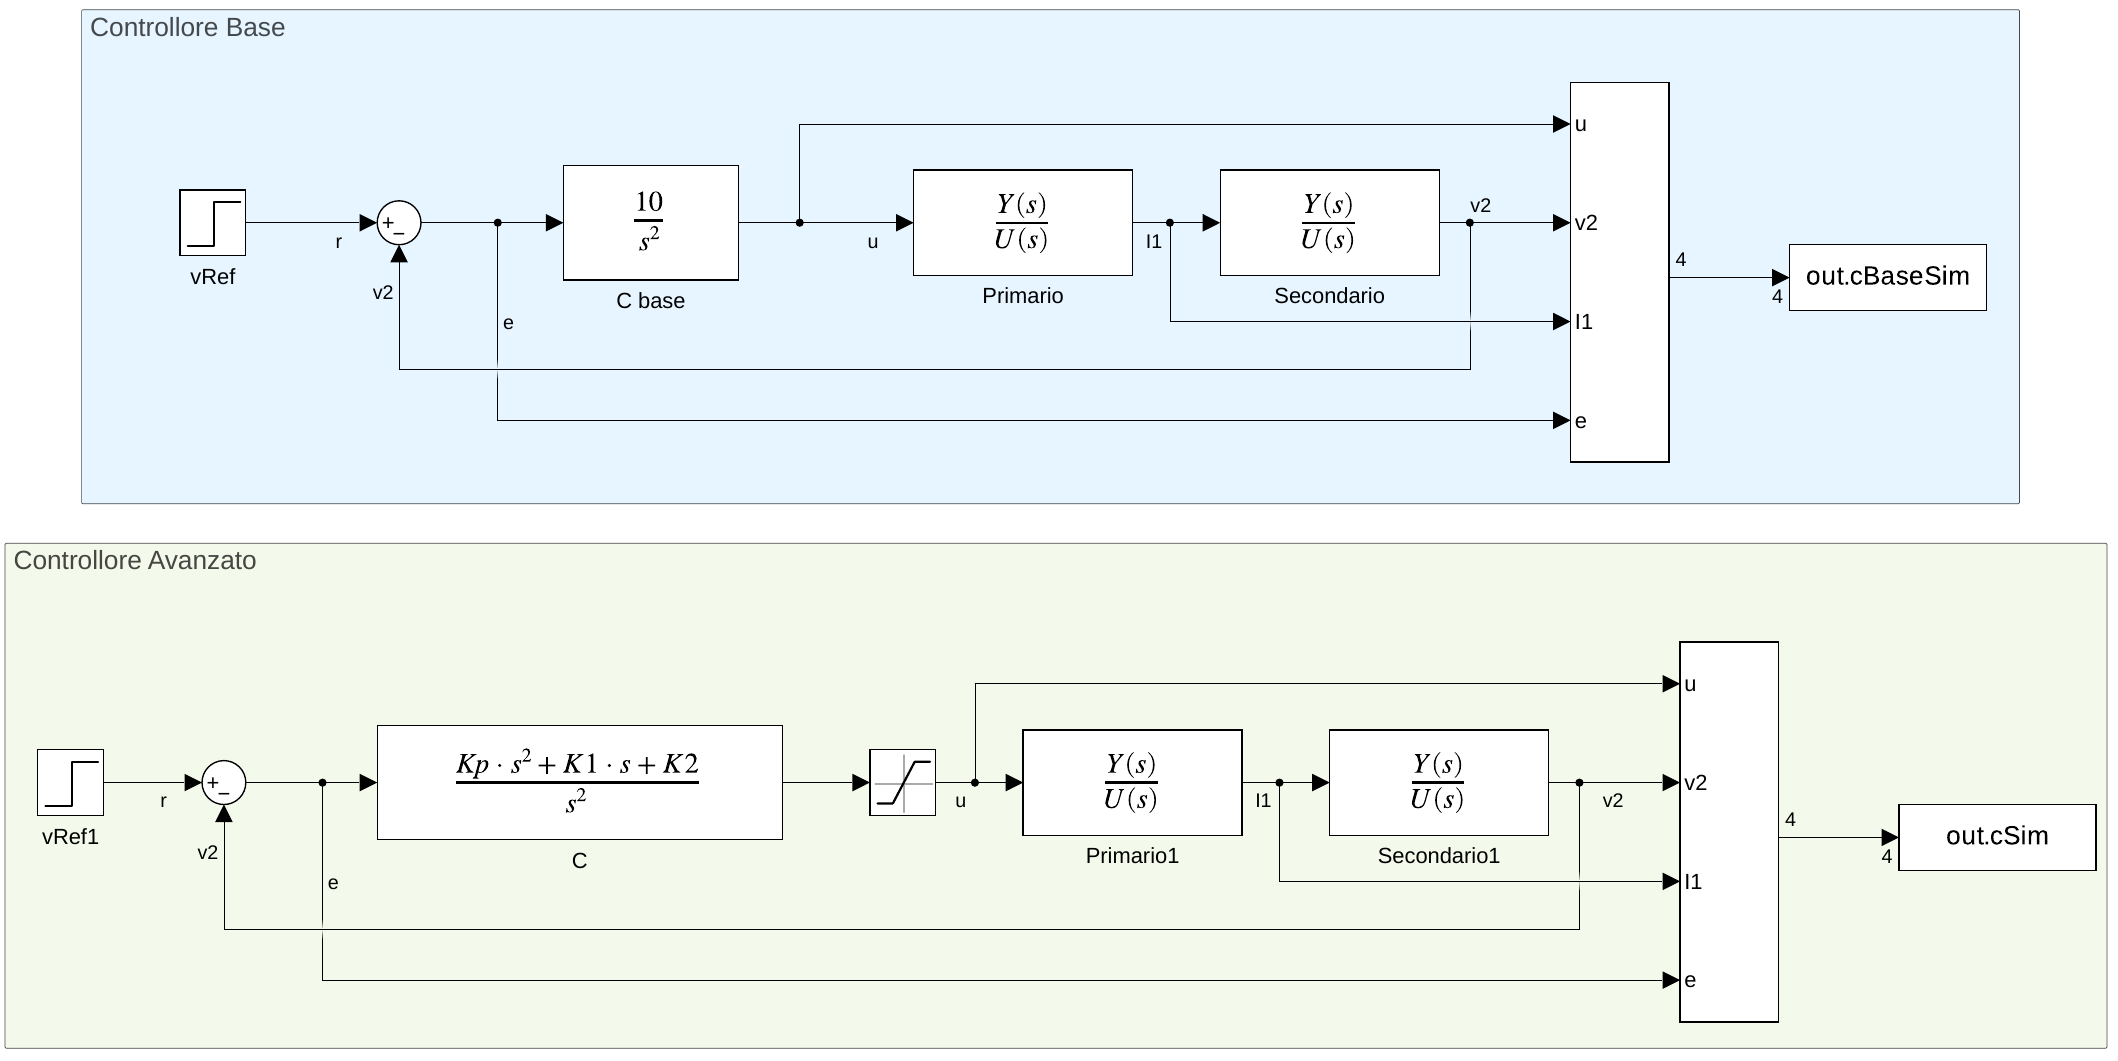
\includegraphics[width=1\textwidth]{ModelloMatematico/systemSimulink.png}
\end{figure}\vspace{-6mm}
\noindent
Il primo loop di controllo  serve per avere una prova simulatava a supporto della teoria e mostrare quindi l'andamento base del sistema.\\
Al contrario il secondo loop di controllo punta ad analizzare la risposta del sistema al variare dei coefficienti con lo scopo preciso di migliorarne le prestazioni.\\
In entrambi i casi, la tensione $ V_{2_{ref}} = 0.5V$\\
\begin{spacing}{1}
	\noindent
	{\footnotesize NOTA BENE: I grafici riportati hanno il \textbf{\underline{segnale di errore zoomato di un fattore 10}} per meglio mettere in evidenza il comportamento dell'errore}
\end{spacing}

\newpage

\subsection{Design Base di controllo}
Usando il controllo base e senza saturazione, abbiamo una risposta che conferma i gli esiti calcolati per $ e_\infty $ nella sezione \ref{eq:esitiErrore}:
\begin{figure}[H]
	\centering
	\caption[Modelli simulati su Simulink]{Modelli simulati su Simulink}
	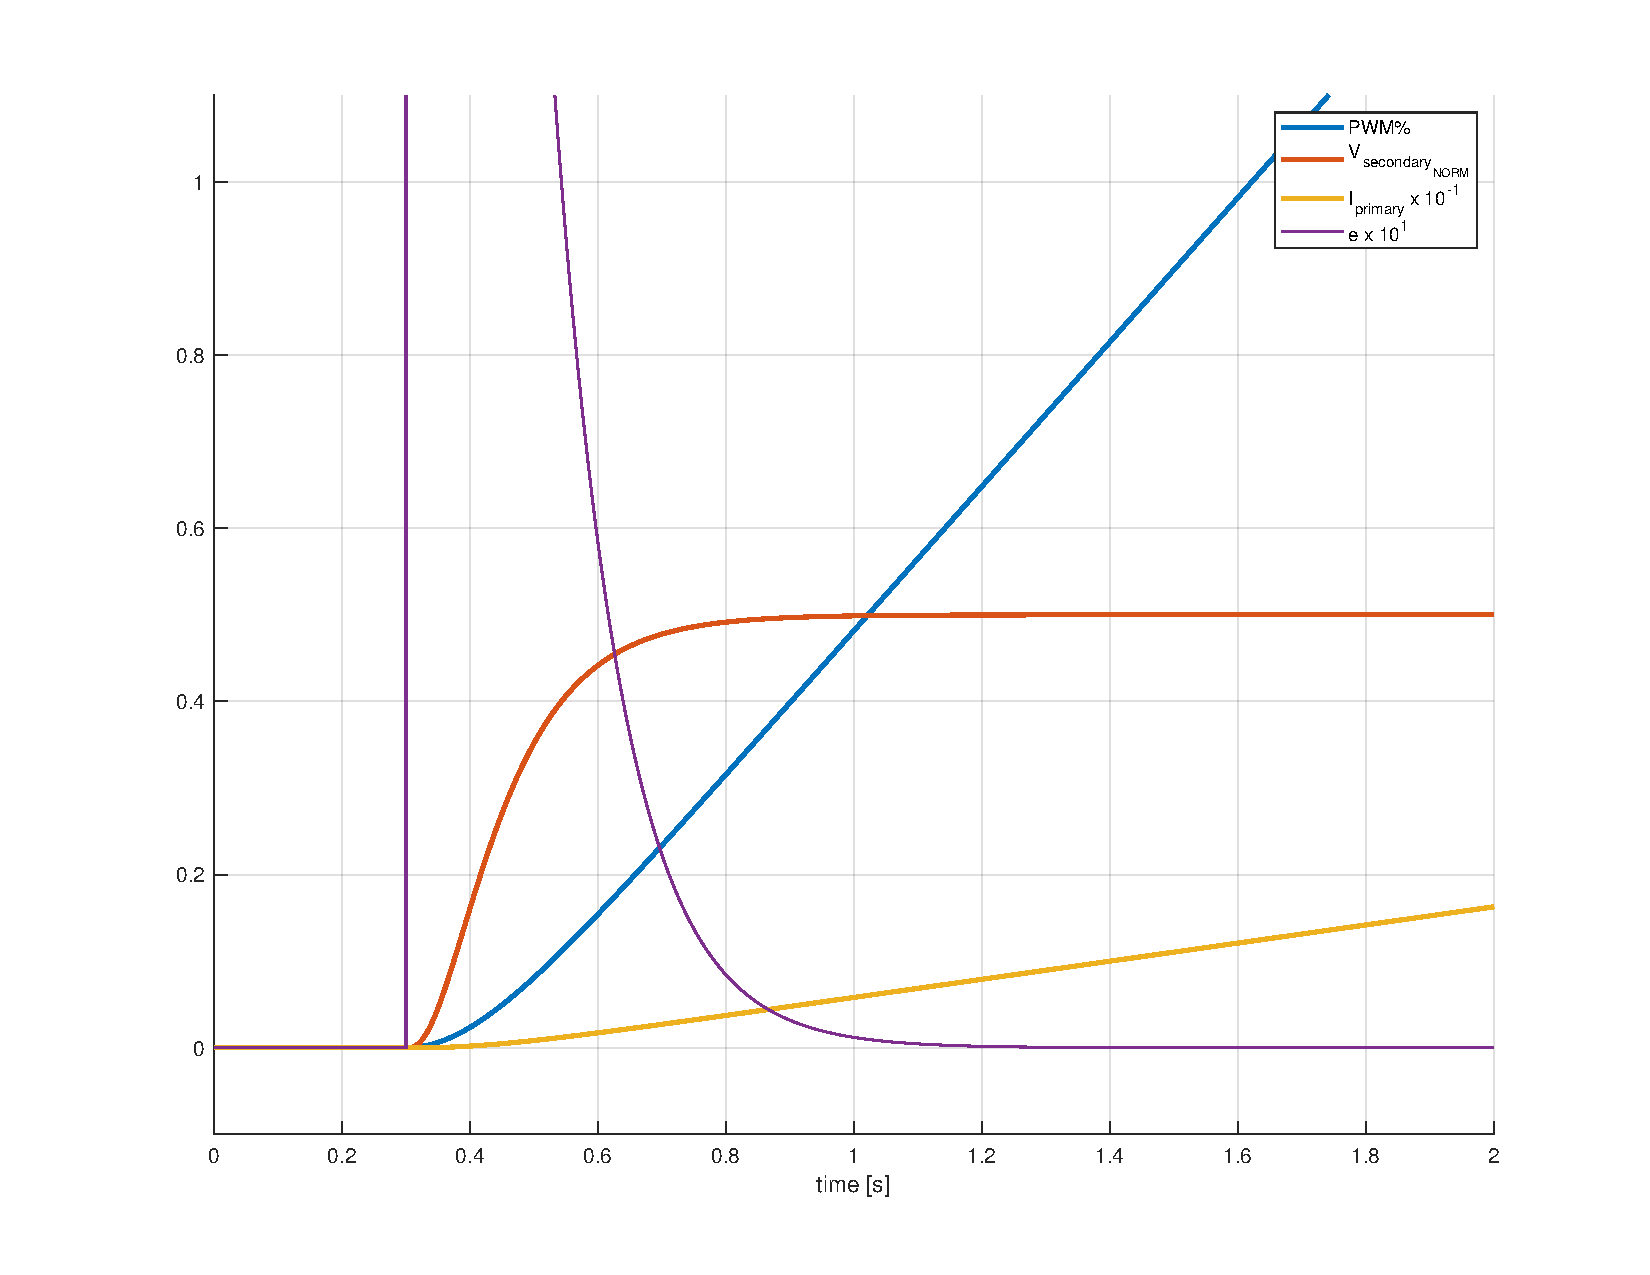
\includegraphics[width=1\textwidth]{ModelloMatematico/Simulation-cBaseSim.pdf}
\end{figure}

\noindent
Queste performance possono e devono essere ampliamene migliorate poiché raggiunta la saturazione del controllo, l'errore ricomincia subito a crescere ed è impossibile riprenderlo senza resettare l'esperimento.\\
In questo caso però la saturazione è stata eliminata al fine di mettere maggiormente in evidenza che asintoticamente il controllo proposto realizza le richieste di controllo di avere un inseguitore con errore nullo asintotico.

\newpage
\subsection{Design Avanzato di controllo}
Usando ora il controllore proposto nell'equazione \ref{eq:controllerDesign} analizziamo ora gli effetti della presenza dei vari termini, e il loro effetto qualitativo sulla risposta e l'andamento dell'errore.\\
Ricordiamo nuovamente che il {\color{red}\textbf{\underline{segnale di errore è zoomato di un fattore 10}}} per meglio mettere in evidenza il comportamento dell'errore.

\subsubsection{Analisi controllo Avanzato per $ K_p $=0 $ K_1 $=0 $ K_2 $=100}
\begin{figure}[H]
	\centering
	\caption[Controllo Avanzato $ K_p $=0 $ K_1 $=0 $ K_2 $=100] {Controllo Avanzato $ K_p $=0 $ K_1 $=0 $ K_2 $=100}
	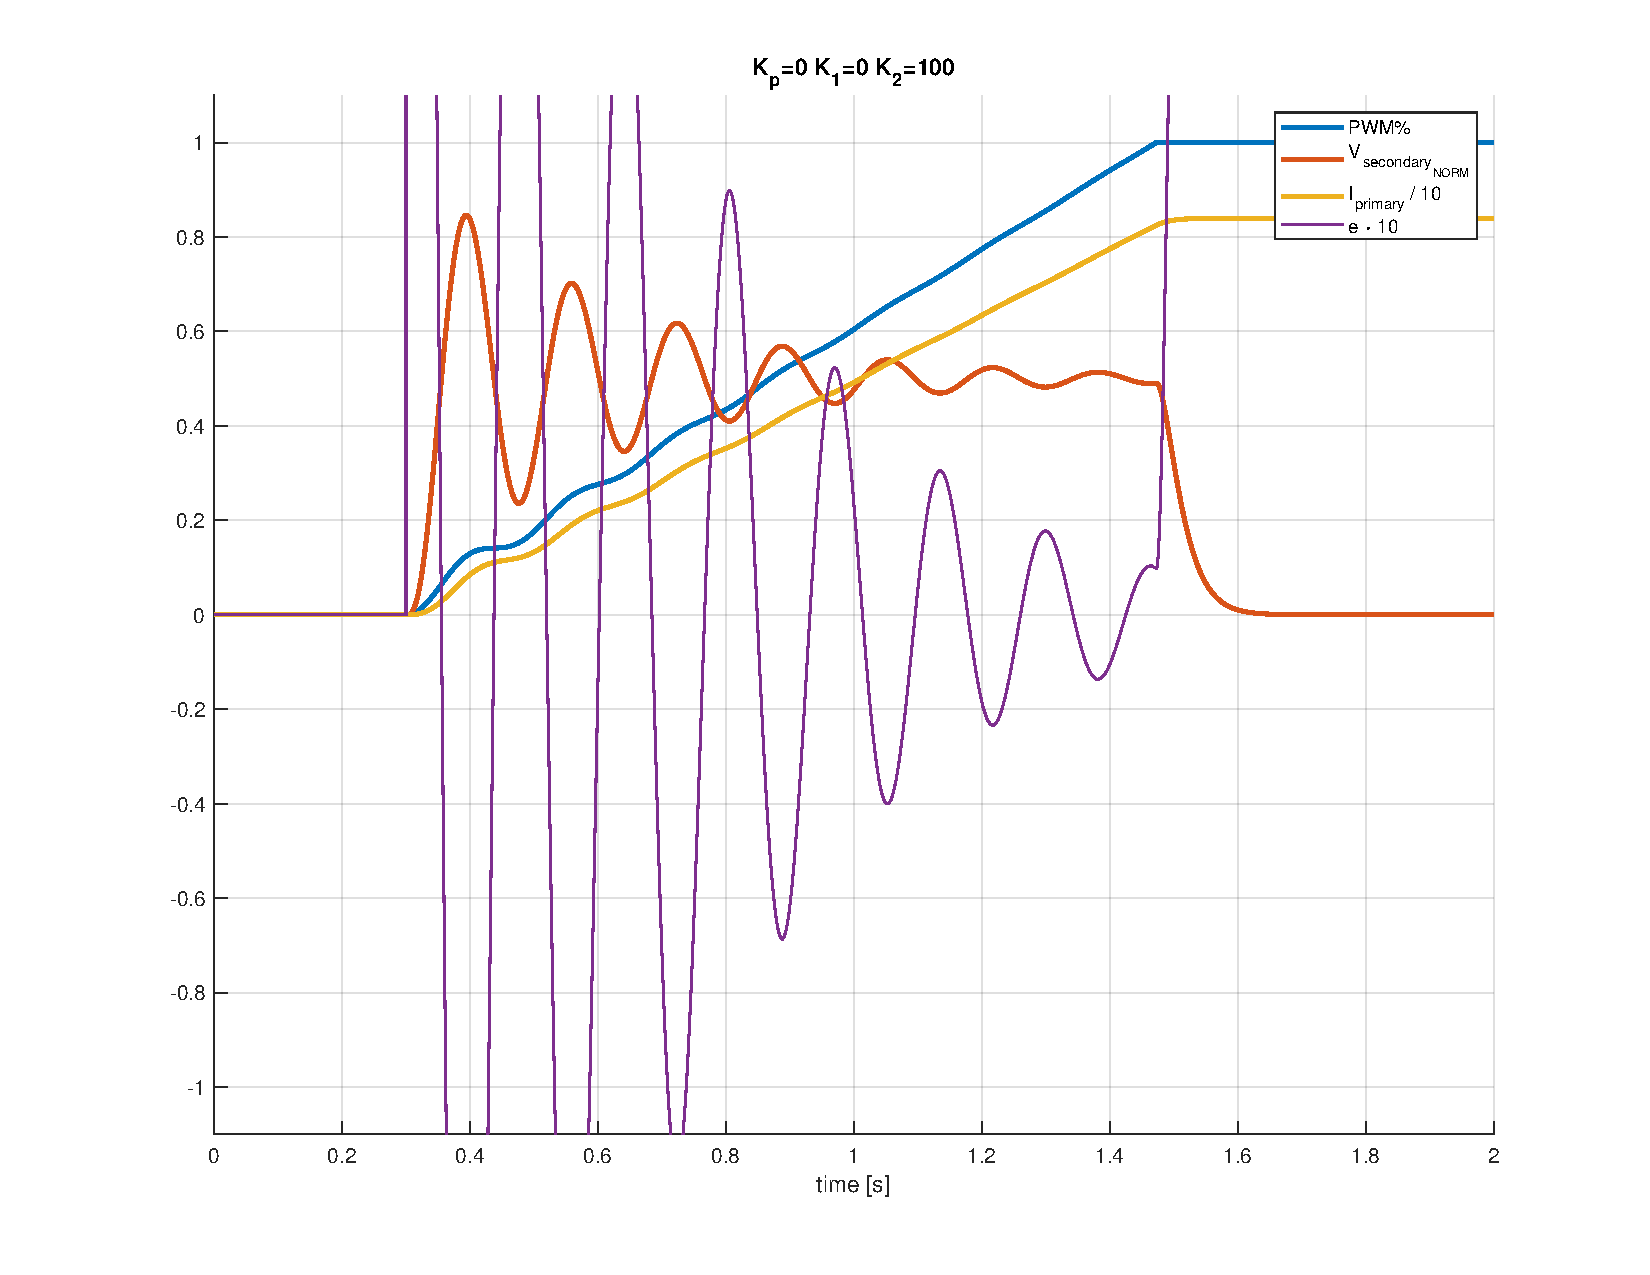
\includegraphics[width=1\textwidth]{ModelloMatematico/Simulation-cSim-K_p=0-K_1=0-K_2=100.pdf}
\end{figure}
\noindent
L'aumento del coefficiente per il doppio integratore ha l'effetto di creare risposte più tempestive, ma da atto a dei fenomeni oscillatori smorzati

\subsubsection{Analisi controllo Avanzato per $ K_p $=0 $ K_1 $=10 $ K_2 $=100}
In questa seconda simulazione si è aggiunto un al controllore il termine integrale:
\begin{figure}[H]
	\centering
	\caption[Controllo Avanzato $ K_p $=0 $ K_1 $=10 $ K_2 $=100]{Controllo Avanzato $ K_p $=0 $ K_1 $=10 $ K_2 $=100}
	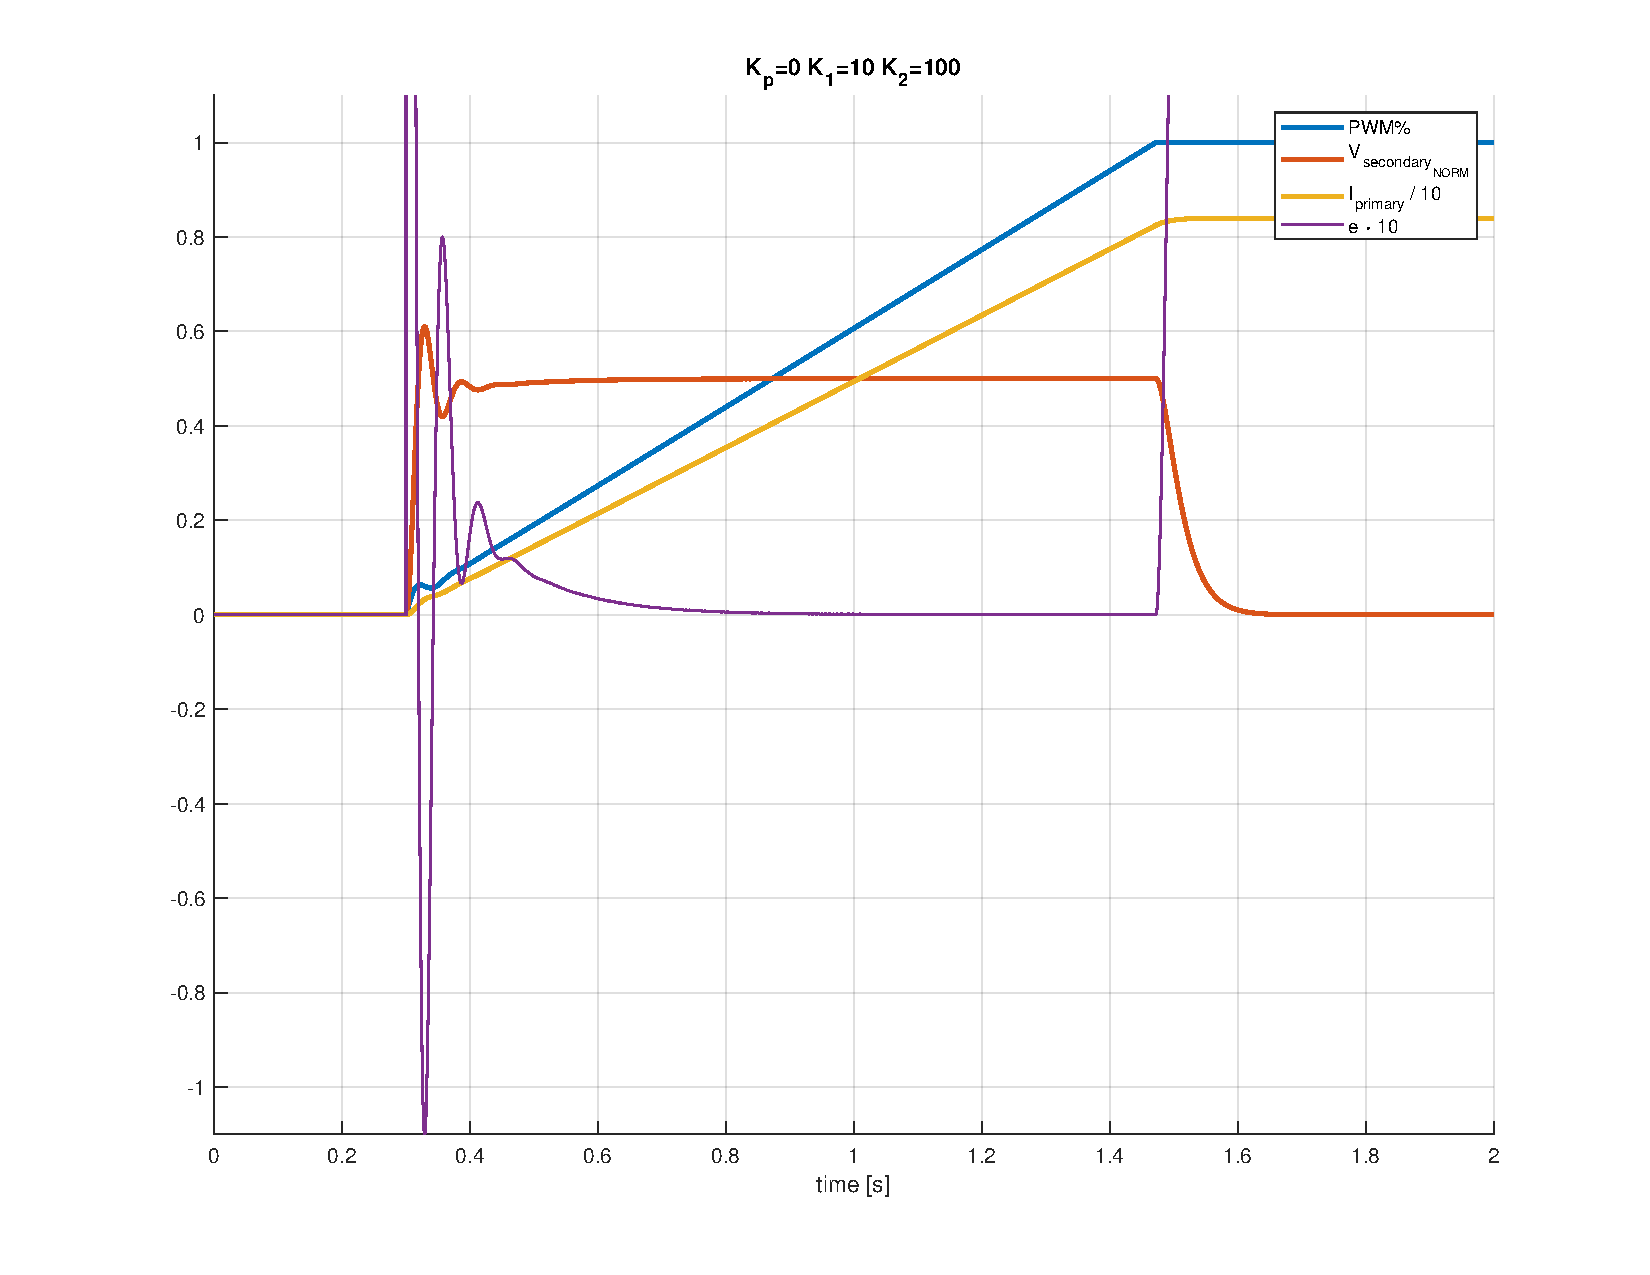
\includegraphics[width=1\textwidth]{ModelloMatematico/Simulation-cSim-K_p=0-K_1=10-K_2=100.pdf}
\end{figure}
\noindent
L'effetto del termine integrale è quindi smorzare il transitorio oscillatorio, per poi inseguire il riferimento con un andamento esponenziale.\\
In questo secondo esperimento abbiamo già migliorato molto le performance dal controllo base, avendo visibilmente migliorato il \underline{Tempo di assestamento} del sistema e lasciando 600ms di esperimento con errore ampiamente trascurabile.
\newpage
\subsubsection{Analisi controllo Avanzato per $ K_p $=0 $ K_1 $=100 $ K_2 $=500}
Abbiamo adesso aumentato i coefficienti del doppio e singolo integratore per vedere come migliorano le performance del sistema ad un loro aumento coordinato:
\begin{figure}[H]
	\centering
	\caption[Controllo Avanzato $ K_p $=0 $ K_1 $=100 $ K_2 $=500]{Controllo Avanzato $ K_p $=0 $ K_1 $=100 $ K_2 $=500}
	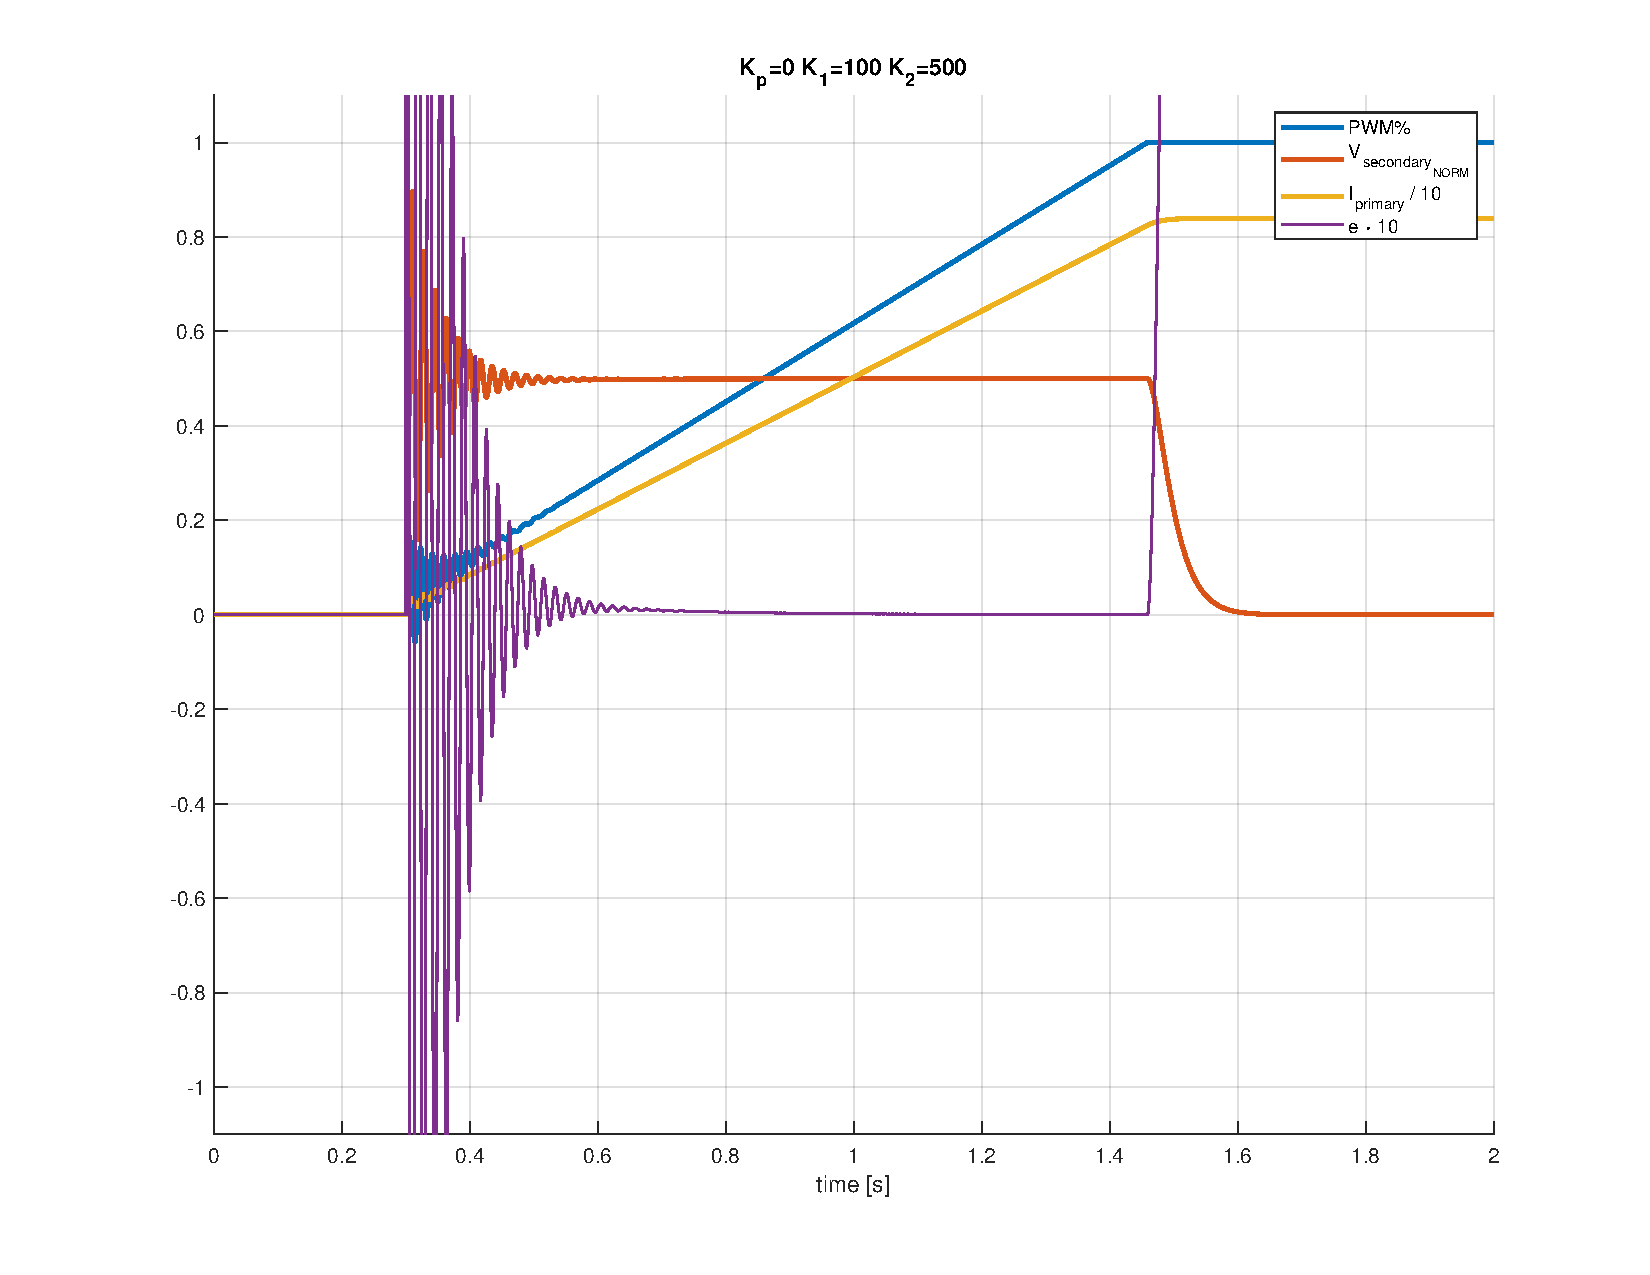
\includegraphics[width=1\textwidth]{ModelloMatematico/Simulation-cSim-K_p=0-K_1=100-K_2=500.pdf}
\end{figure}
\noindent
L'effetto è un ulteriore miglioramento sul \underline{Tempo di assestamento} e una una discesa più pronunciata dell'errore verso lo 0, ma abbiamo pagato questo incremento prestazionale con il ritorno degli effetti oscillatori smorzati, ed essi sono anche a frequenze maggiori, non proprio desiderabile.

\newpage

\subsubsection{Analisi controllo Avanzato per $ K_p $=0.2 $ K_1 $=100 $ K_2 $=500}
Aggiungiamo quindi al caso precedente un termine proporzionale all'errore, così da rispondere subito alle variazioni del riferimento:
\begin{figure}[H]
	\centering
	\caption[Controllo Avanzato $ K_p $=0.2 $ K_1 $=100 $ K_2 $=500]{Controllo Avanzato $ K_p $=0.2 $ K_1 $=100 $ K_2 $=500}
	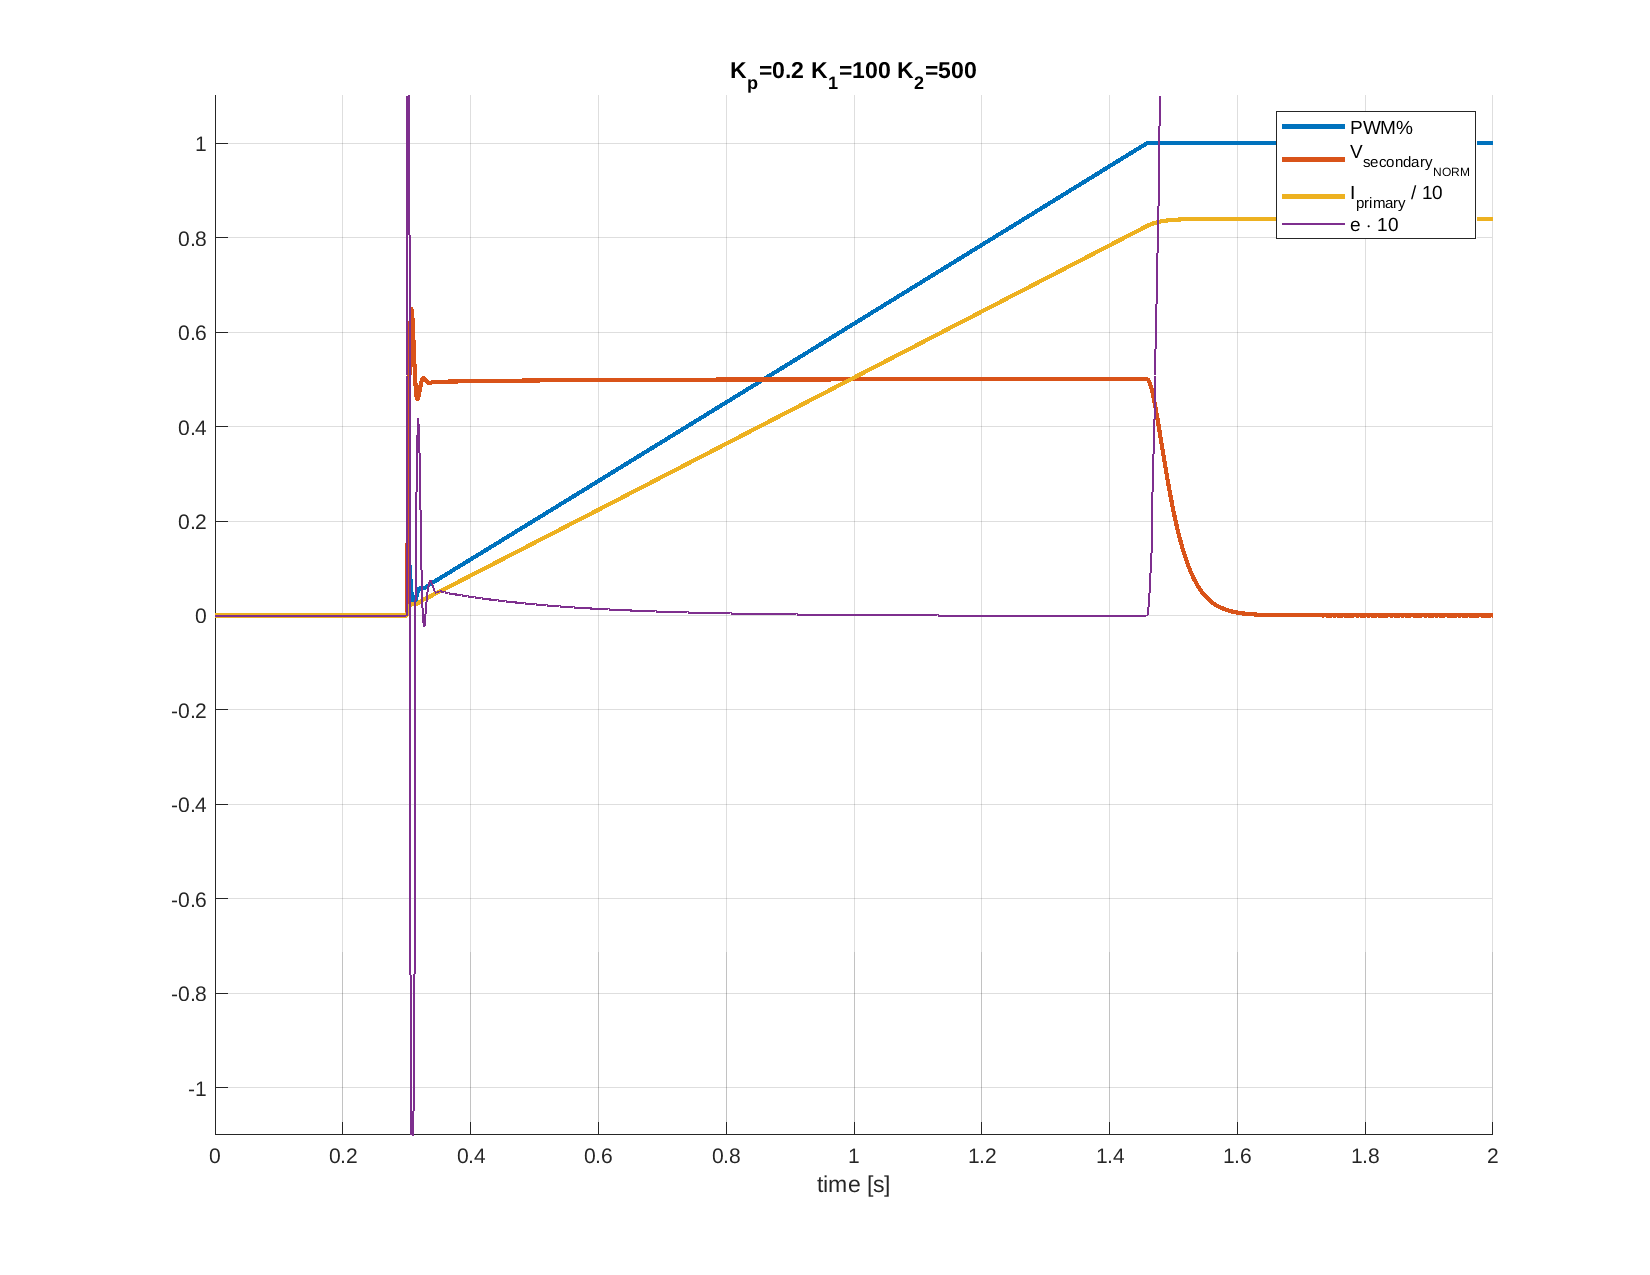
\includegraphics[width=1\textwidth]{ModelloMatematico/Simulation-cSim-K_p=0.2-K_1=100-K_2=500}
\end{figure}
\noindent
Essendo $ K_p $ istantaneo con la variazione del riferimento, abbiamo che l'inseguimento di $ V_{2_{ref}} $ inizia prima, riducendo il margine di fase dovuto al caricamento degli integratori, ciò riduce il fenomeno di wind-up presente precedentemente e causa delle oscillazioni attorno al riferimento, e permette di tornare al comportamento del 2° esperimento, con performance nettamente superiori.

\newpage

\subsubsection{Analisi controllo Avanzato per $ K_p $=0.8 $ K_1 $=100 $ K_2 $=500}
In quest'ultimo esperimento analizziamo l'effetto dell'aumento del termine proporzionale sulla dinamica:
\begin{figure}[H]
	\centering
	\caption[Controllo Avanzato $ K_p $=0.8 $ K_1 $=100 $ K_2 $=500]{Controllo Avanzato $ K_p $=0.8 $ K_1 $=100 $ K_2 $=500}
	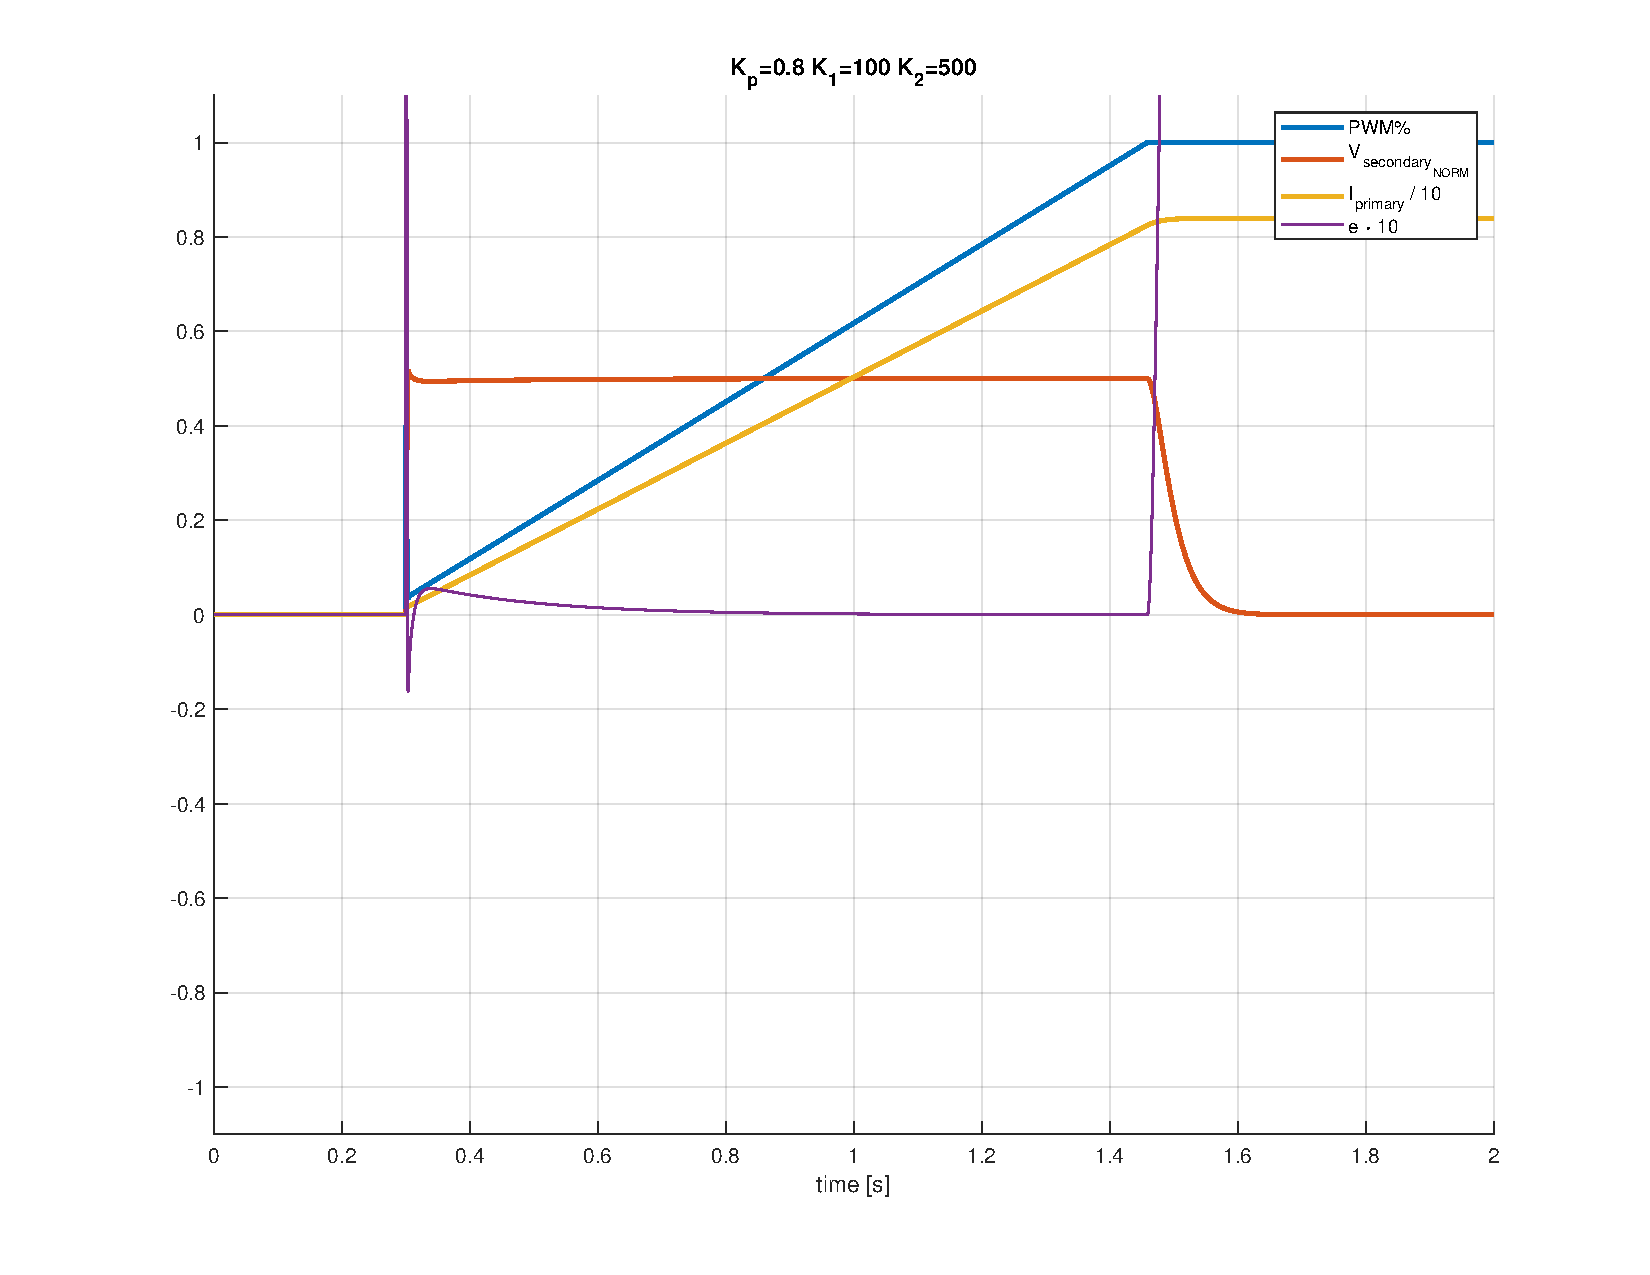
\includegraphics[width=1\textwidth]{ModelloMatematico/Simulation-cSim-K_p=0.8-K_1=100-K_2=500.pdf}
\end{figure}
\noindent
Rispetto al caso precedente, l'errore iniziale si è molto ridotto, passando da un fuori scala in entrambi i segni, a un errore di $ -0.019V $ di picco negativo (il picco positivo è per definizione $ 0.5V $ essendo il riferimento dato come gradino).\\
Al contrario, superata questa prima fase, il resto della dinamica è fondamentalmente identica al caso precedente, indice che $ K_p $ serve solo per rispondere alle prime variazioni.

\newpage

\section{Conclusioni per il design Avanzato} \label{sec:designControlloreConclusioni}
In conclusione possiamo dire che il controllore "\textit{PID-style}" definito nell'equazione \ref{eq:controllerDesign} permette di ottenere gli obiettivi di controllo prefissati a prescindere dai coefficienti usati, e la possibilità di raggiungere delle performance di tutto rispetto ottimizzando opportunamente i coefficienti.\\
Qui di seguito una descrizione qualitativa degli effetti da aspettarsi con una loro variazione:
\begin{description}
	\item[{\boldmath$ K_2 $}] Permette di raggiungere gli obiettivi di inseguimento con errore nullo, un suo aumento migliora la risposta ma causa delle oscillazioni smorzate a frequenze via via più elevate. \\
	      $\Rightarrow$ \textbf{Raggiungimento degli obiettivi di controllo}
	\item[{\boldmath$ K_1 $}] Se dimensionato opportunamente rende più marcato lo smorzamento delle oscillazioni dovute a $ K_2 $ fino a tornare ad un andamento esponenziale.\\
	      $\Rightarrow$ \textbf{Migliora Tempo di Assestamento}
	\item[{\boldmath$ K_p $}] Migliorare le performance nei primi istanti di controllo, prima che gli integratori possano arrivare a convergenza.\\
	      $\Rightarrow$ \textbf{Miglioramento del Tempo di risposta}
\end{description} \vspace{-8mm}
\noindent
\begin{center}
	\rule{0.75\linewidth}{0.5px}
\end{center}\vspace{-4mm}
\noindent
I valori dei coefficienti visti in simulazione e calcolati sul modello però non possono essere implementati 1:1 nel caso reale, a causa delle \nonLinearita che sono state trascurate nella creazione del modello, uniti ai problemi dovuti al tempo di campionamento e attuazione del sistema che è pari a $ 2Khz $, i quali se scelti troppo elevati portano a fastidiosi effetti oscillatori attorno l'errore nullo.\\
Non di meno, le osservazioni qui riportate continuano ad essere valide anche sul sistema reale, ed essendo le \nonLinearita presenti soprattutto nei pressi della \textit{Dead-zone} e della \textit{Saturazione} e di bassa intensità, essi possono essere modellati come del disturbo non troppo ampio, e si vede dagli esperimenti reali che il controllore così progettato è anche robusto per questo tipo di errori di attuazione.



